\documentclass{article}
\usepackage[utf8]{inputenc}
\usepackage[T1]{fontenc}
\usepackage{geometry}
\usepackage{enumitem}
\usepackage{graphicx}
\usepackage{multicol}

\geometry{margin=0.5in}

\begin{document}

\title{\textbf{Sprawozdanie i specyfikacja projektu}
\\ \large{\textit{Ganics}}}
\author{\textbf{Adrian Chmiel}}
\date{9 czerwca 2024}
\maketitle

\textbf{Link do repozytorium:} \textit{https://github.com/chmieladr/Ganics}

\section{Cel projektu}
Celem projektu jest wykorzystanie sieci GAN do generowania obrazów z przetłumaczonym stylem. Program oferuje dwie możliwe opcje konwersji stylu:
\begin{enumerate}[label=\arabic*.]
    \setlength\itemsep{0pt}
    \item \textbf{Sztuka Vincenta Van Gogha} - obrazy będą przypominać dzieła Vincenta Van Gogha
    \item \textbf{Kreskówka} - obrazy będą przypominać obrazy z kreskówek (lub komiksów)
\end{enumerate}
Po przetłumaczeniu stylu obraz jest upscalowany do rozdzielczości \textit{512x512}. Ostateczny obraz jest zapisywany w formacie \textit{.png}.

\section{Wykorzystane technologie}
Program został napisany w języku \textbf{Python 3.10}. Wykorzystuje następujące biblioteki:
\begin{itemize}
    \setlength\itemsep{0pt}
    \item \textbf{matplotlib} - do tworzenia wykresów i wizualizacji danych
    \item \textbf{numpy} - do operacji na macierzach
    \item \textbf{opencv-python} - do przetwarzania obrazów
    \item \textbf{pandas} - do analizy danych
    \item \textbf{pillow} - do przetwarzania obrazów
    \item \textbf{pydot} - do wizualizacji struktury modelu
    \item \textbf{tensorflow} - do tworzenia i trenowania modeli GAN
    \item \textbf{tkinter} - do stworzenia prostego interfejsu graficznego
    \item \textbf{tqdm} - do wyświetlania postępu w trenowaniu modelu
\end{itemize}
Wybrałem język programowania Python, ponieważ jest powszechnie używany w dziedzinie uczenia maszynowego i sztucznej inteligencji. Oferuje szeroki zakres bibliotek i narzędzi, które ułatwiają realizację takich projektów. Spośród wielu bibliotek do uczenia maszynowego wybrałem \textbf{Tensorflow}, ponieważ jest jedną z najpopularniejszych bibliotek do tworzenia sieci neuronowych i korzystałem z niej już wcześniej w ramach innych projektach.
\vspace{3mm} \\
Dla tego projektu zdecydowałem się na użycie wersji \textbf{Python 3.10} głównie dlatego, że jest to ostatnia wersja wspierana przez \textit{Tensorflow 2.10}. Nowe wersje tej biblioteki nie obsługują natywnie akceleracji GPU na systemie operacyjnym \textbf{Windows}, co jest kluczowe dla procesu uczenia, ponieważ znacznie skraca czas potrzebny na trenowanie sieci. Mimo że mógłbym ograniczyć projekt do systemów \textit{Linux}, chciałem uczynić go bardziej dostępnym.
\vspace{3mm} \\
Oprócz tego wykorzystałem \textbf{Jupyter Notebooks} do trenowania modeli. Ich główną zaletą jest możliwość uruchamiania kodu w małych fragmentach, co ułatwia znalezienie problemów i zrozumienie kodu. Są dostępne w katalogu \textit{notebooks}.

\section{Uruchomienie programu}
Aby uruchomić aplikację bezpośrednio z \textbf{kodu źródłowego}, zaleca się utworzenie nowego środowiska wirtualnego i zainstalowanie wymaganych bibliotek/pakietów w nim.
Zakładając, że korzystamy z \textit{condy}, możemy to zrobić za pomocą następujących poleceń:
\begin{verbatim}
conda create -n Ganics python=3.10 -y
conda activate Ganics
conda install jupyter -y
pip install -r requirements.txt
\end{verbatim}
\textit{Instalację Jupyter można pominąć, jeśli nie planujemy korzystać z notebooków.}
\vspace{3mm} \\
Dla posiadaczy kart graficznych \textit{NVIDIA} warto również uruchomić poniższe polecenie, które umożliwi korzystanie z \textit{CUDA} (pod warunkiem, że zainstalowano inne niezbędne oprogramowanie):
\begin{verbatim}
conda install -c conda-forge cudatoolkit=11.2 cudnn=8.1.0 -y
\end{verbatim}
Program można uruchomić, wywołując plik \textbf{\textit{main.py}}:
\begin{verbatim}
python src/main.py
\end{verbatim}
Program został przetestowany na systemach operacyjnych \textit{Windows} i \textit{Linux}.

\section{Interfejs graficzny}
\begin{multicols}{2}
Interfejs graficzny programu został stworzony przy użyciu biblioteki \textit{tkinter}. Pozwala on na:
\begin{itemize}
    \setlength\itemsep{0pt}
    \item Wybór pliku wejściowego
    \item Wybór stylu konwersji
    \item Konwersję i zapisanie obrazu
    \item Podgląd obrazu przed i po konwersji
\end{itemize}
Przykładowy zrzut ekranu interfejsu użytkownika jest widoczny po prawej stronie.
\vspace{5\baselineskip} \\
\columnbreak
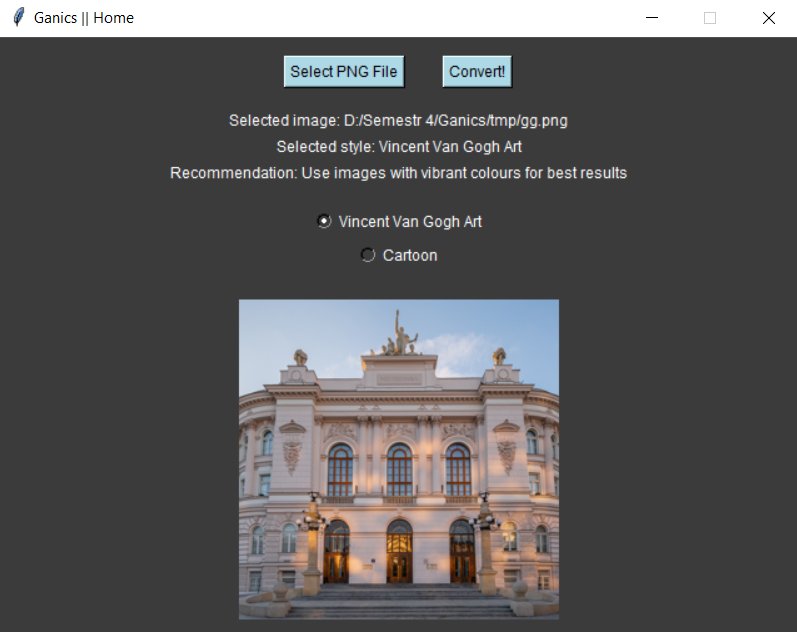
\includegraphics[width=0.475\textwidth]{../imgs/gui.png}
\end{multicols}

\section{Pliki wejściowe i wyjściowe}
\begin{enumerate}[label=\arabic*.]
    \item \textbf{Aplikacja główna} \\
Program pozwala na wybranie ścieżki do pliku wejściowego, który zostanie przekonwertowany. Warto zauważyć, że plik wejściowy musi być obrazem w formacie \textit{.jpg}, \textit{.jpeg} lub \textit{.png}.
\vspace{3mm} \\
Plik wyjściowy, niezależnie od początkowego formatu, zawsze jest obrazem w formacie \textit{.png} o rozdzielczości \textit{512x512}.
    \item \textbf{Notebooki} \\
W przypadku notebooków dostarczamy całe zestawy obrazów jako dane wejściowe (więcej informacji poniżej), które zostaną wykorzystane do trenowania modelu. Jako wynik otrzymujemy wizualizacje ilustrujące działanie modelu po trenowaniu oraz wyeksportowany plik wag modelu, który jest później wykorzystywany jako składnik aplikacji głównej.
\end{enumerate}

\section{Działanie aplikacji}
Poniżej przedstawiono koncepcję działania aplikacji:
\begin{enumerate}[label=\arabic*.]
    \item Wybór pliku i stylu konwersji
    \item Przetłumaczenie stylu obrazu za pomocą \textbf{CycleGAN} \\ \textit{Otrzymany obraz ma rozdzielczość 256x256.}
    \item Upscaling obrazu za pomocą \textbf{SRGAN} do rozdzielczości 512x512
    \item Zapisanie obrazu w formacie \textit{.png}
\end{enumerate}
Ważnym faktem jest, że aplikacja \textbf{nie będzie działać}, jeśli nie znajdzie odpowiednich wag modelu, o czym użytkownik zostanie poinformowany błędem.
W takim przypadku konieczne jest albo uruchomienie notebooków do trenowania modelu, albo pobranie gotowych plików dostępnych na \textit{Google Drive} pod linkiem w pliku \textit{how\_to\_get\_models.md}.

\section{Teoria}
Program opiera się na dwóch modelach sieci GAN:
\begin{itemize}
    \setlength\itemsep{0pt}
    \item \textbf{CycleGAN}
    \item \textbf{SRGAN} (z dyskryminatorem \textit{PatchGAN})
\end{itemize}
\textbf{GAN} \textit{(Generative Adversarial Network)} to rodzaj sztucznej sieci neuronowej, która składa się z dwóch modeli: \textbf{generatora} i \textbf{dyskryminatora}.
Zadaniem generatora jest generowanie nowych obrazów podobnych do tych z zestawu danych, podczas gdy zadaniem dyskryminatora jest rozróżnianie, czy obraz pochodzi od generatora, czy od zestawu danych.
Proces trenowania polega na rywalizacji obu modeli, gdzie generator próbuje oszukać dyskryminator, a dyskryminator próbuje nauczyć się rozróżniania obrazów.
W rezultacie generator jest w stanie generować obrazy bardzo podobne do tych z zestawu danych.

\section{Zbiory danych}
Aby uzyskać zbiory danych do trenowania modeli, można wypakować dostępne pliki \textit{.zip}, które zawierają obrazy przeze mnie wybrane z poniższych zbiorów danych. Alternatywną opcją jest skorzystanie z linków do tych zbiorów dostępnych w pliku \textit{README.md}.
Dzięki temu podejściu można samodzielnie wybrać obrazy, które zostaną wykorzystane do trenowania.
\vspace{3mm} \\
Zbiory danych wykorzystane do trenowania modeli to:
\begin{itemize}
    \item \textbf{Familyguy} (z zestawu danych Cartoon Classification) \\
Użyty do trenowania CycleGAN odpowiedzialnego za konwersję stylu na kreskówkę (lub komiks).
    \item \textbf{VincentVanGogh} (z zestawu danych Vincent Van Gogh Art) \\
Użyty do trenowania kolejnego CycleGAN odpowiedzialnego za konwersję stylu na dzieła Vincenta Van Gogha.
    \item \textbf{natural\_images} \\
Przykładowe obrazy, których styl został przekształcony na jeden z dwóch wyżej wymienionych podczas trenowania modeli.
    \item \textbf{mscoco}
Zbiór danych, który dodatkowo rozszerzył zestaw danych z obrazami naturalnymi wykorzystanymi do trenowania modeli.
\end{itemize}

\section{Ograniczenia}
Konwersja stylu jest zadaniem stosunkowo skomplikowanym, dlatego czas trenowania w notebookach silnie zależy od mocy obliczeniowej komputera. Z tego powodu zaleca się korzystanie z karty graficznej \textit{NVIDIA}, która znacznie przyspiesza proces nauki. Wszystkie notebooki są dostosowane do korzystania z \textit{CUDA}, jeśli jest dostępne, czyli wymagane oprogramowanie zostało zainstalowane.
\vspace{3mm} \\
Warto również zauważyć, że styl kreskówki jest stosunkowo prosty, więc model podczas konwersji obrazów obetnie detale. W przypadku zbyt skomplikowanych obrazów rezultat może być niezadowalający.

\section{Wizualizacja modeli}
Na kolejnych stronach widoczne są wizualizacje modeli wykorzystanych w aplikacji. Wizualizacje te zostały wygenerowane za pomocą biblioteki \textit{pydot}. Pokazują zarówno generator, jak i dyskryminator obu modeli, wraz z poszczególnymi warstwami i ich połączeniami. Więcej informacji dostępnych jest w dokumencie \textit{Notes.pdf}.
\newpage

\begin{multicols}{2}
\subsection{CycleGAN - Generator \vspace{0.25\baselineskip}}
    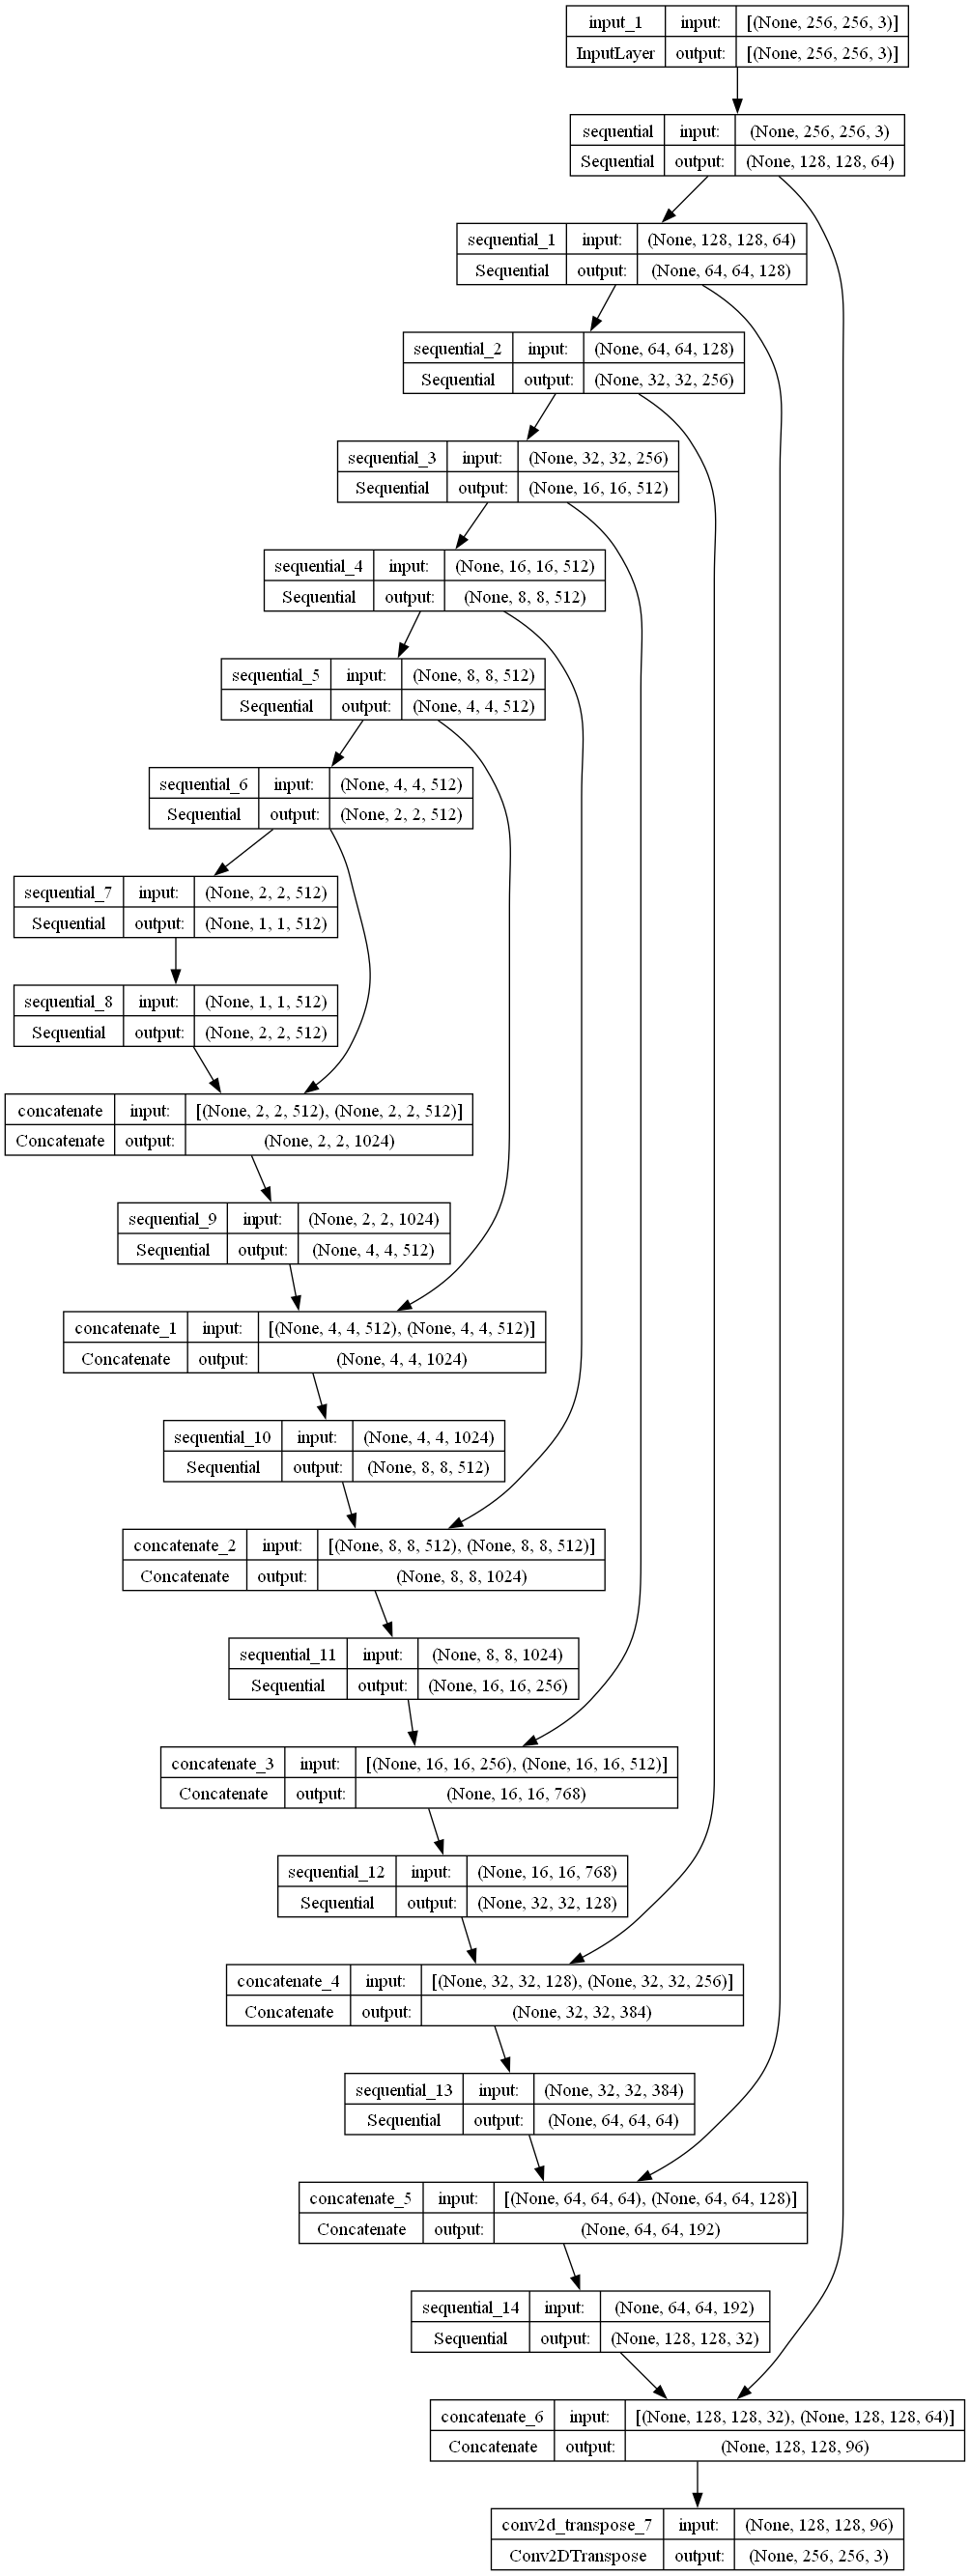
\includegraphics[width=0.475\textwidth]{../imgs/cyclegan_generator.png}
\subsection{CycleGAN - Dyskryminator}
    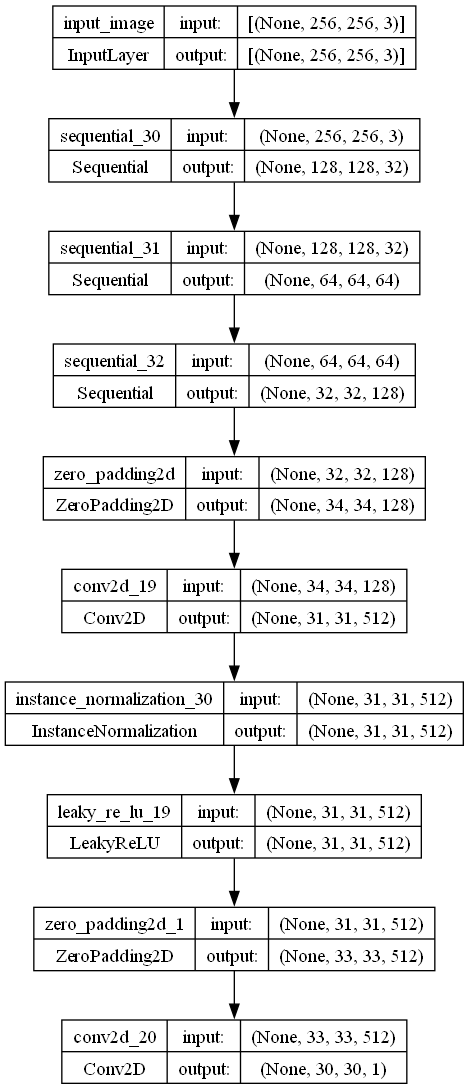
\includegraphics[width=0.475\textwidth]{../imgs/cyclegan_discriminator.png}
\end{multicols}
\newpage

\begin{multicols}{2}
\subsection{SRGAN - Generator \vspace{1.25\baselineskip}}
    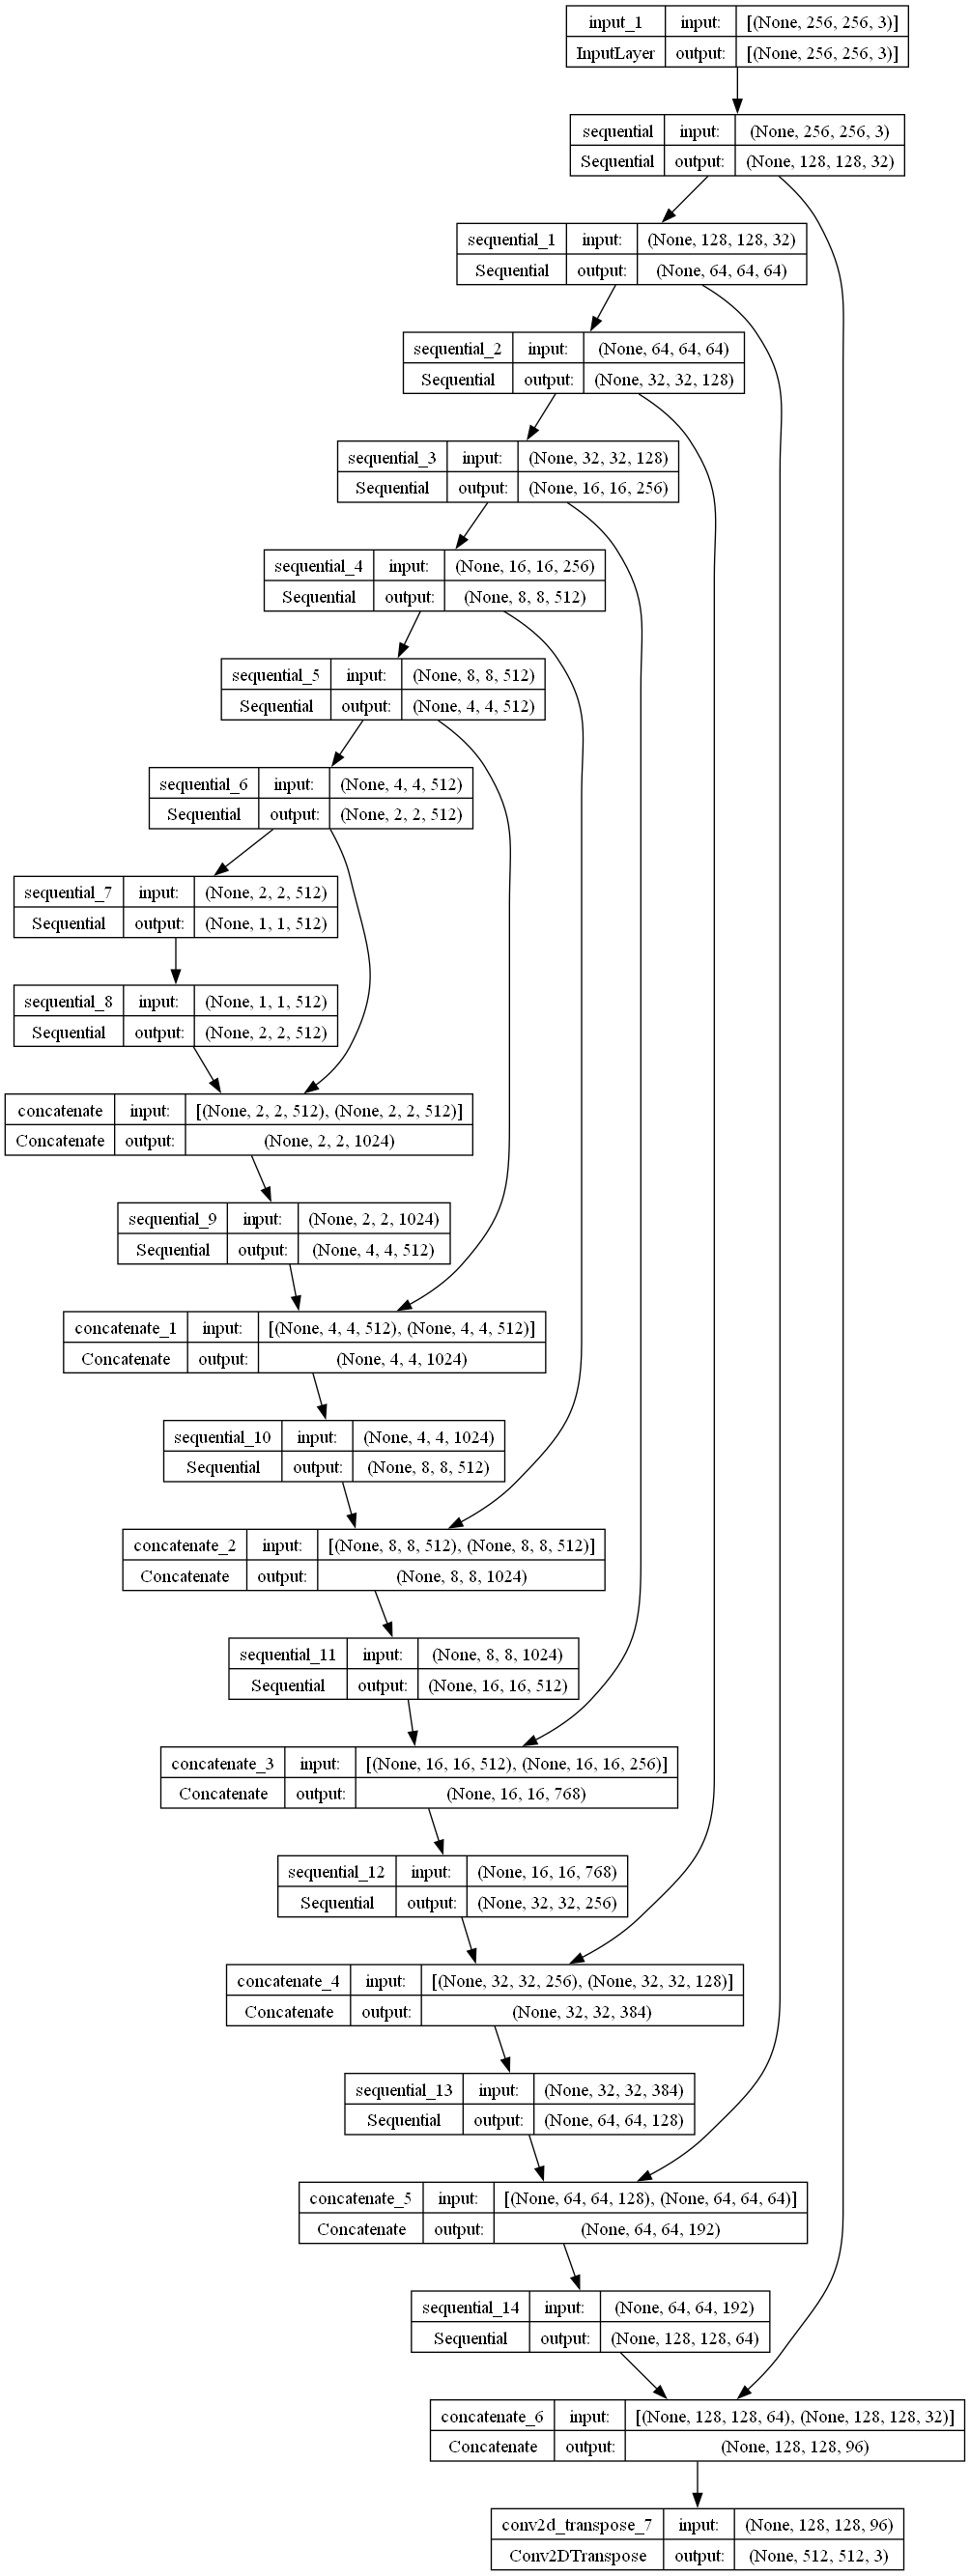
\includegraphics[width=0.475\textwidth]{../imgs/srgan_generator.png}
\subsection{SRGAN - Dyskryminator \\ \textit{(PatchGAN)}}
    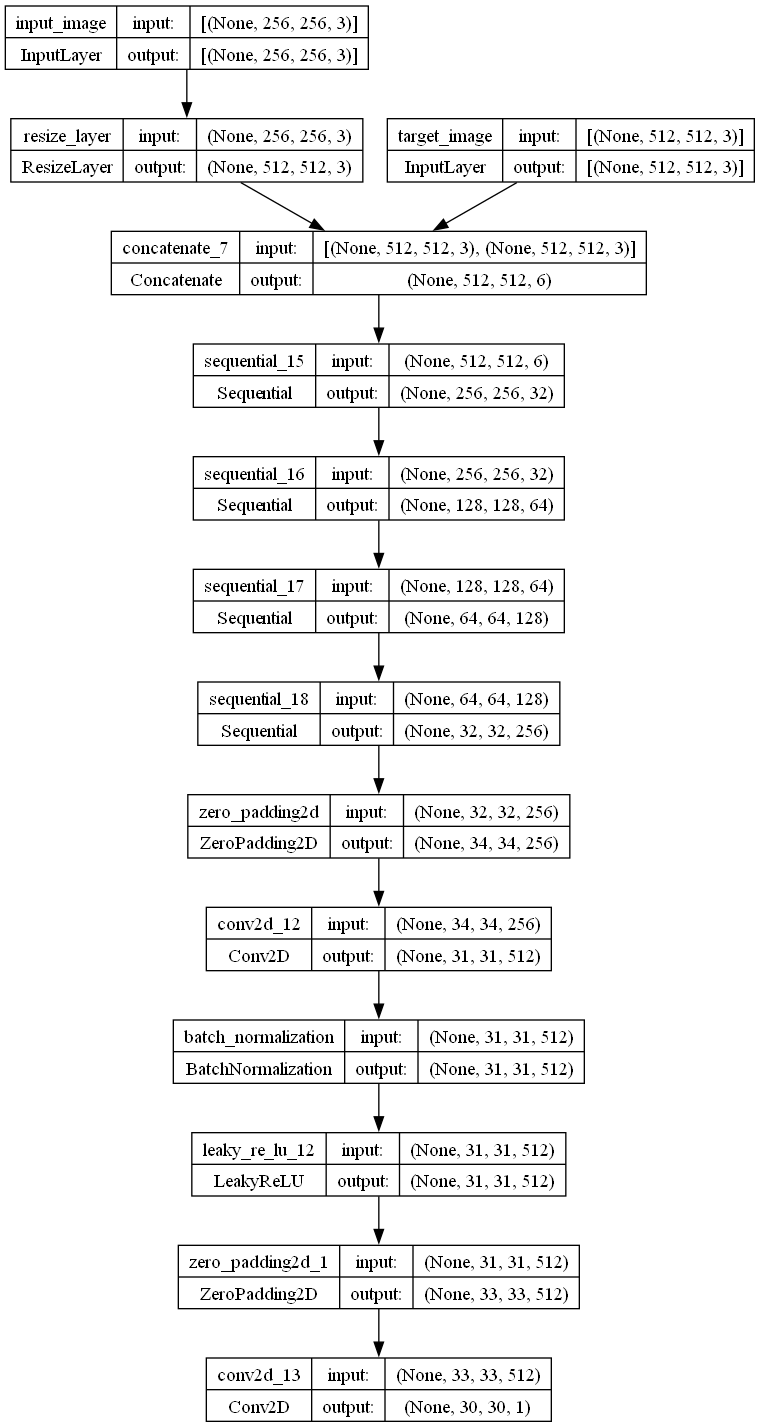
\includegraphics[width=0.475\textwidth]{../imgs/srgan_discriminator.png}
\end{multicols}
\newpage

\section{Przykładowe wyniki}
Poniżej można zobaczyć przykładowe obrazy wyeksportowane z aplikacji. Obrazy po lewej stronie to obrazy wejściowe, a obrazy po prawej stronie to wyniki konwersji.

\subsection{Sztuka Vincent Van Gogha}
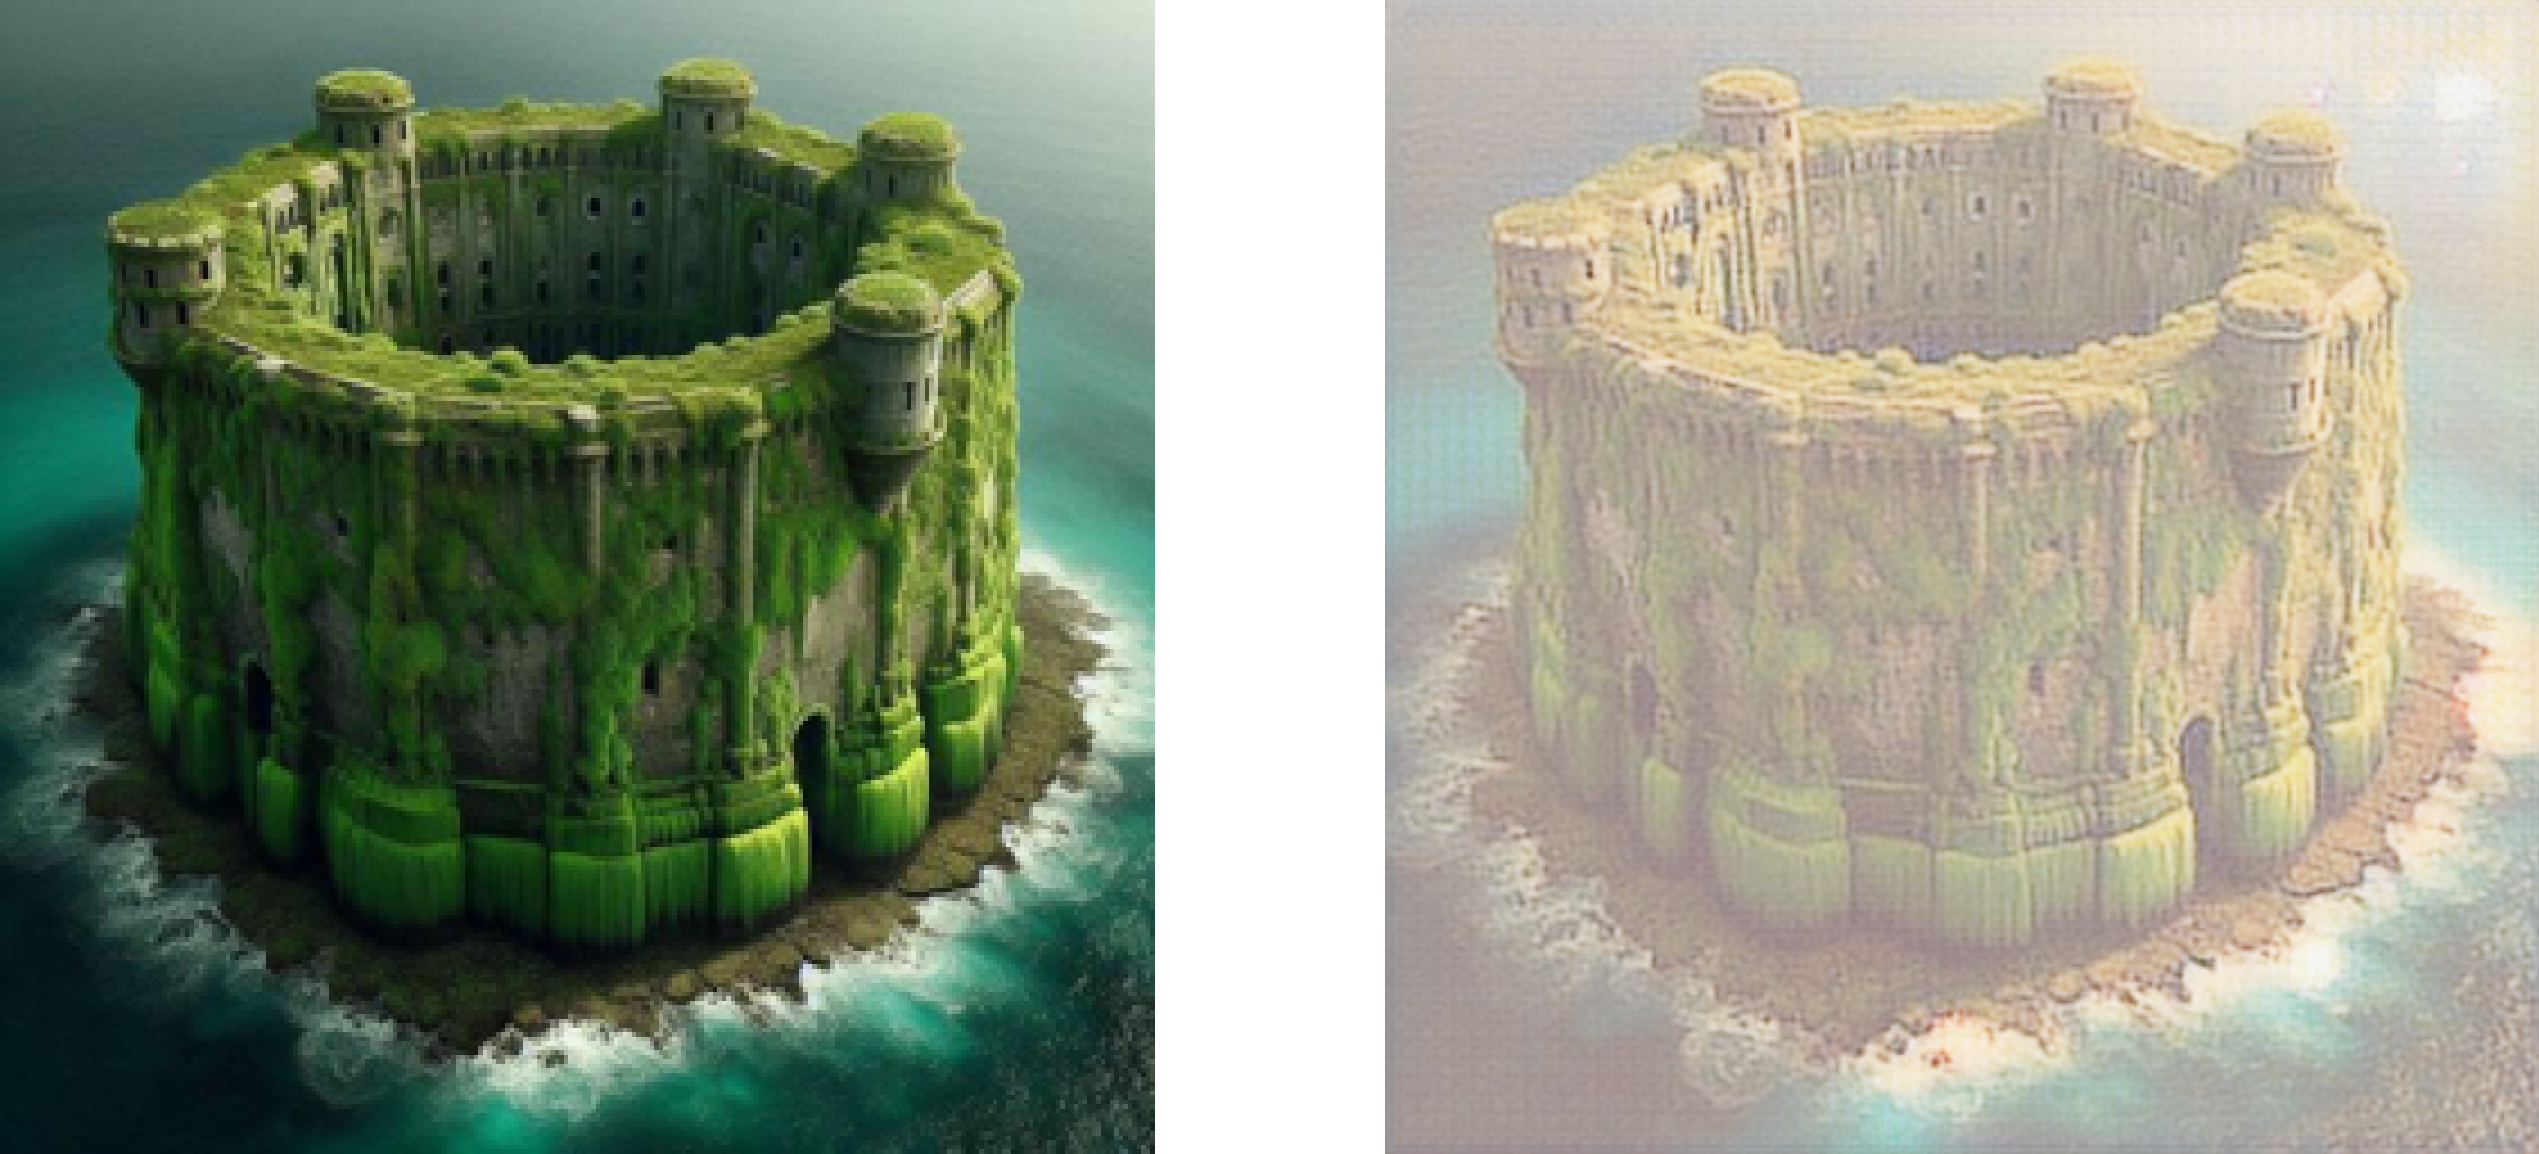
\includegraphics[width=\textwidth]{../imgs/side_by_side/v1.png}
\vspace{3mm} \\
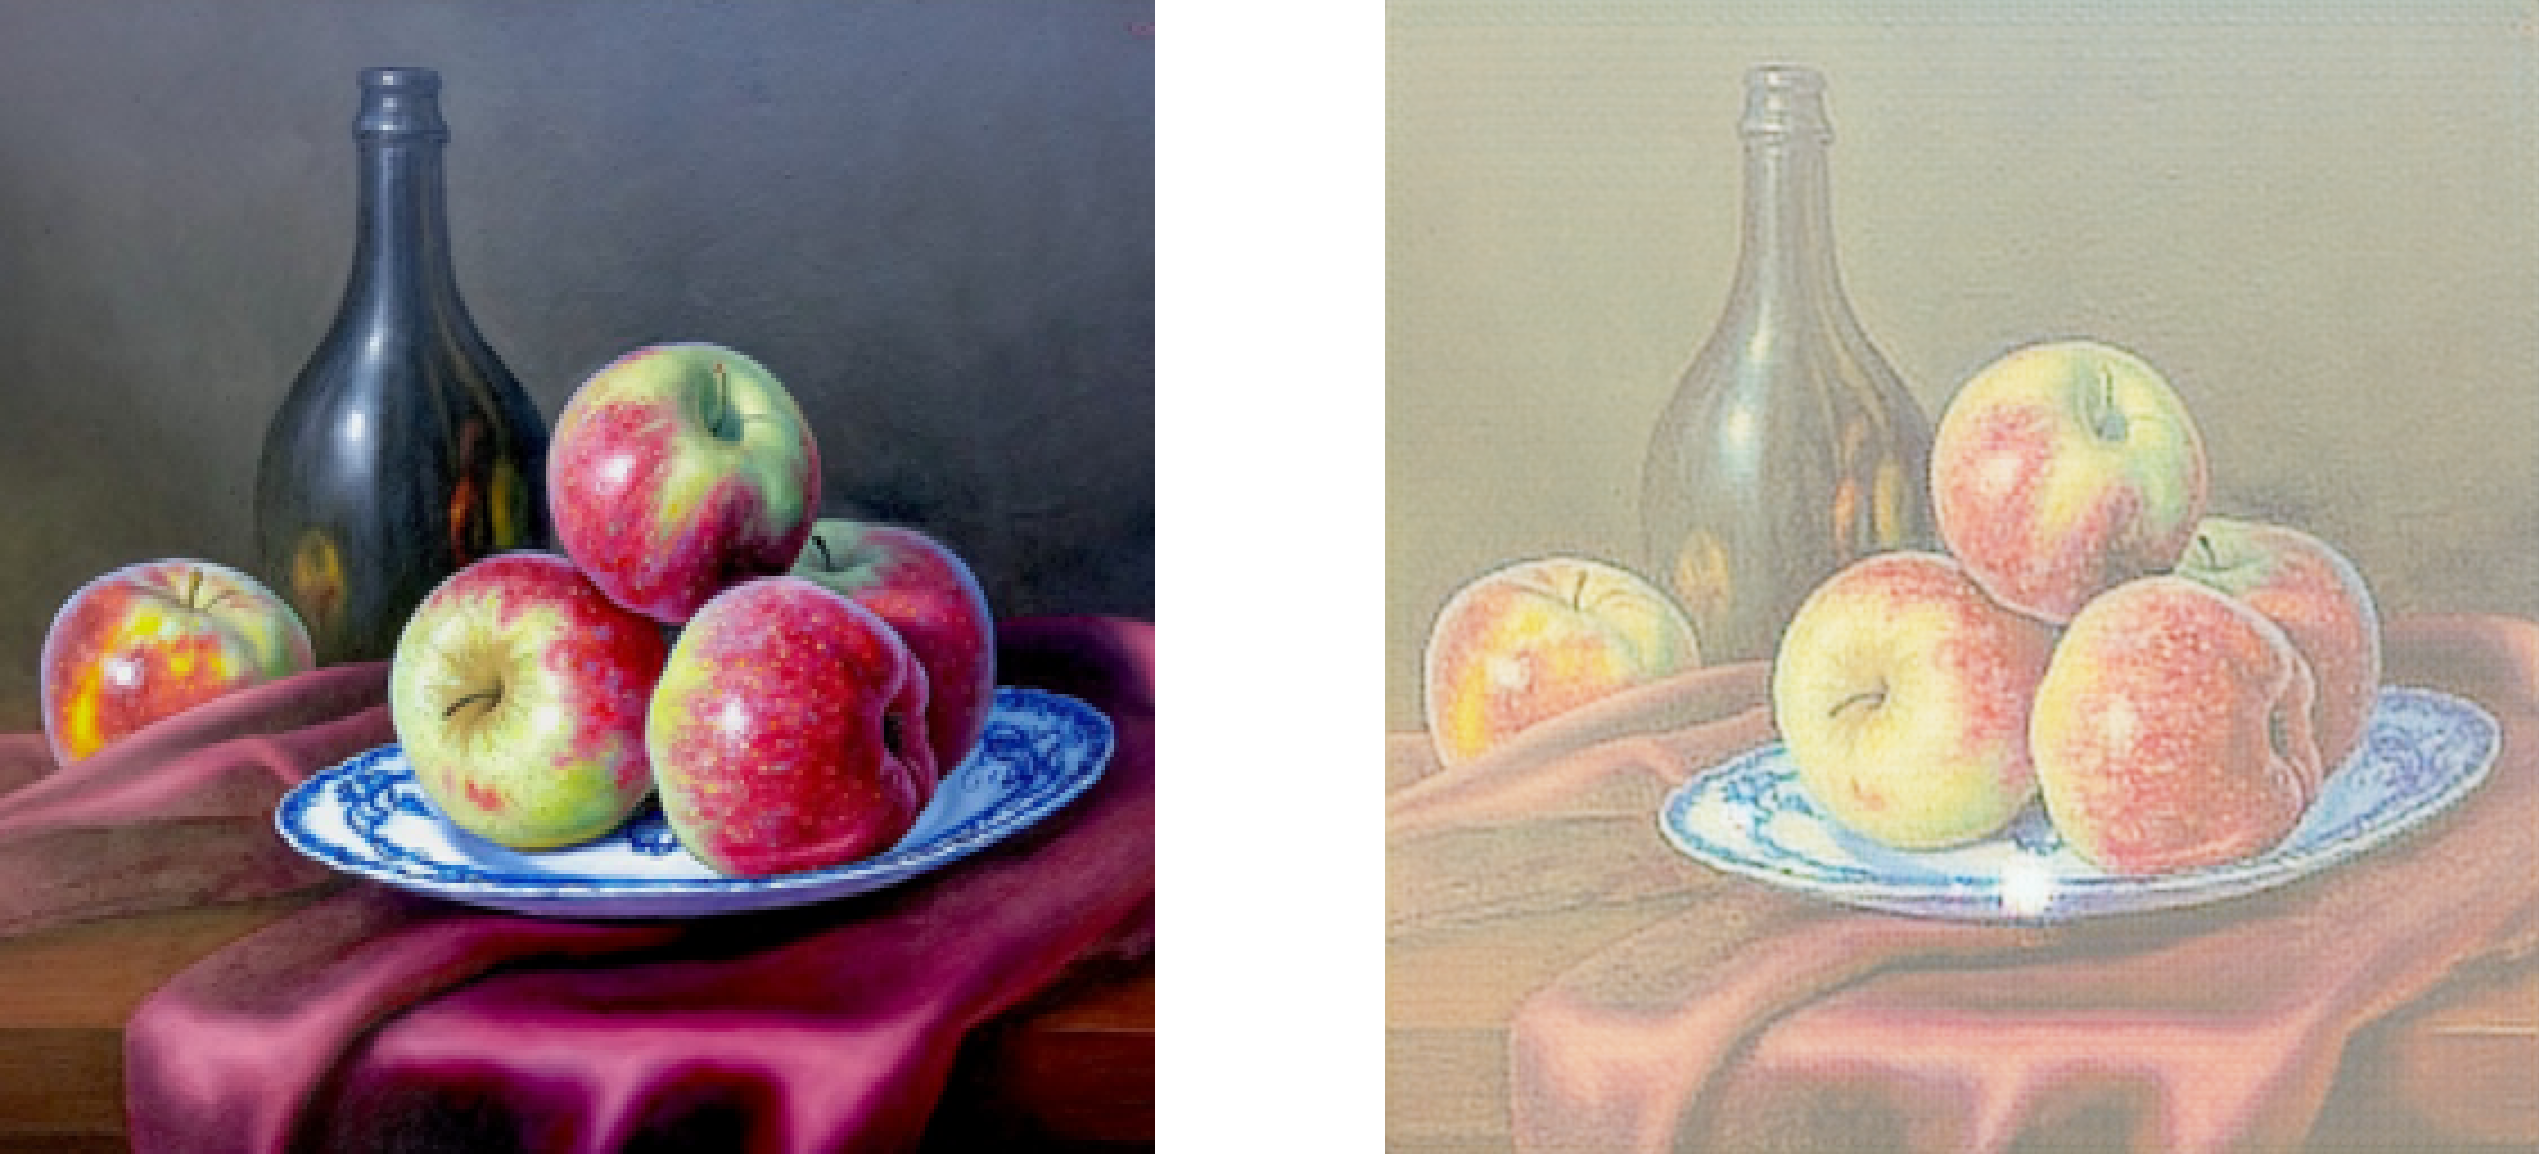
\includegraphics[width=\textwidth]{../imgs/side_by_side/v2.png}
\vspace{3mm} \\
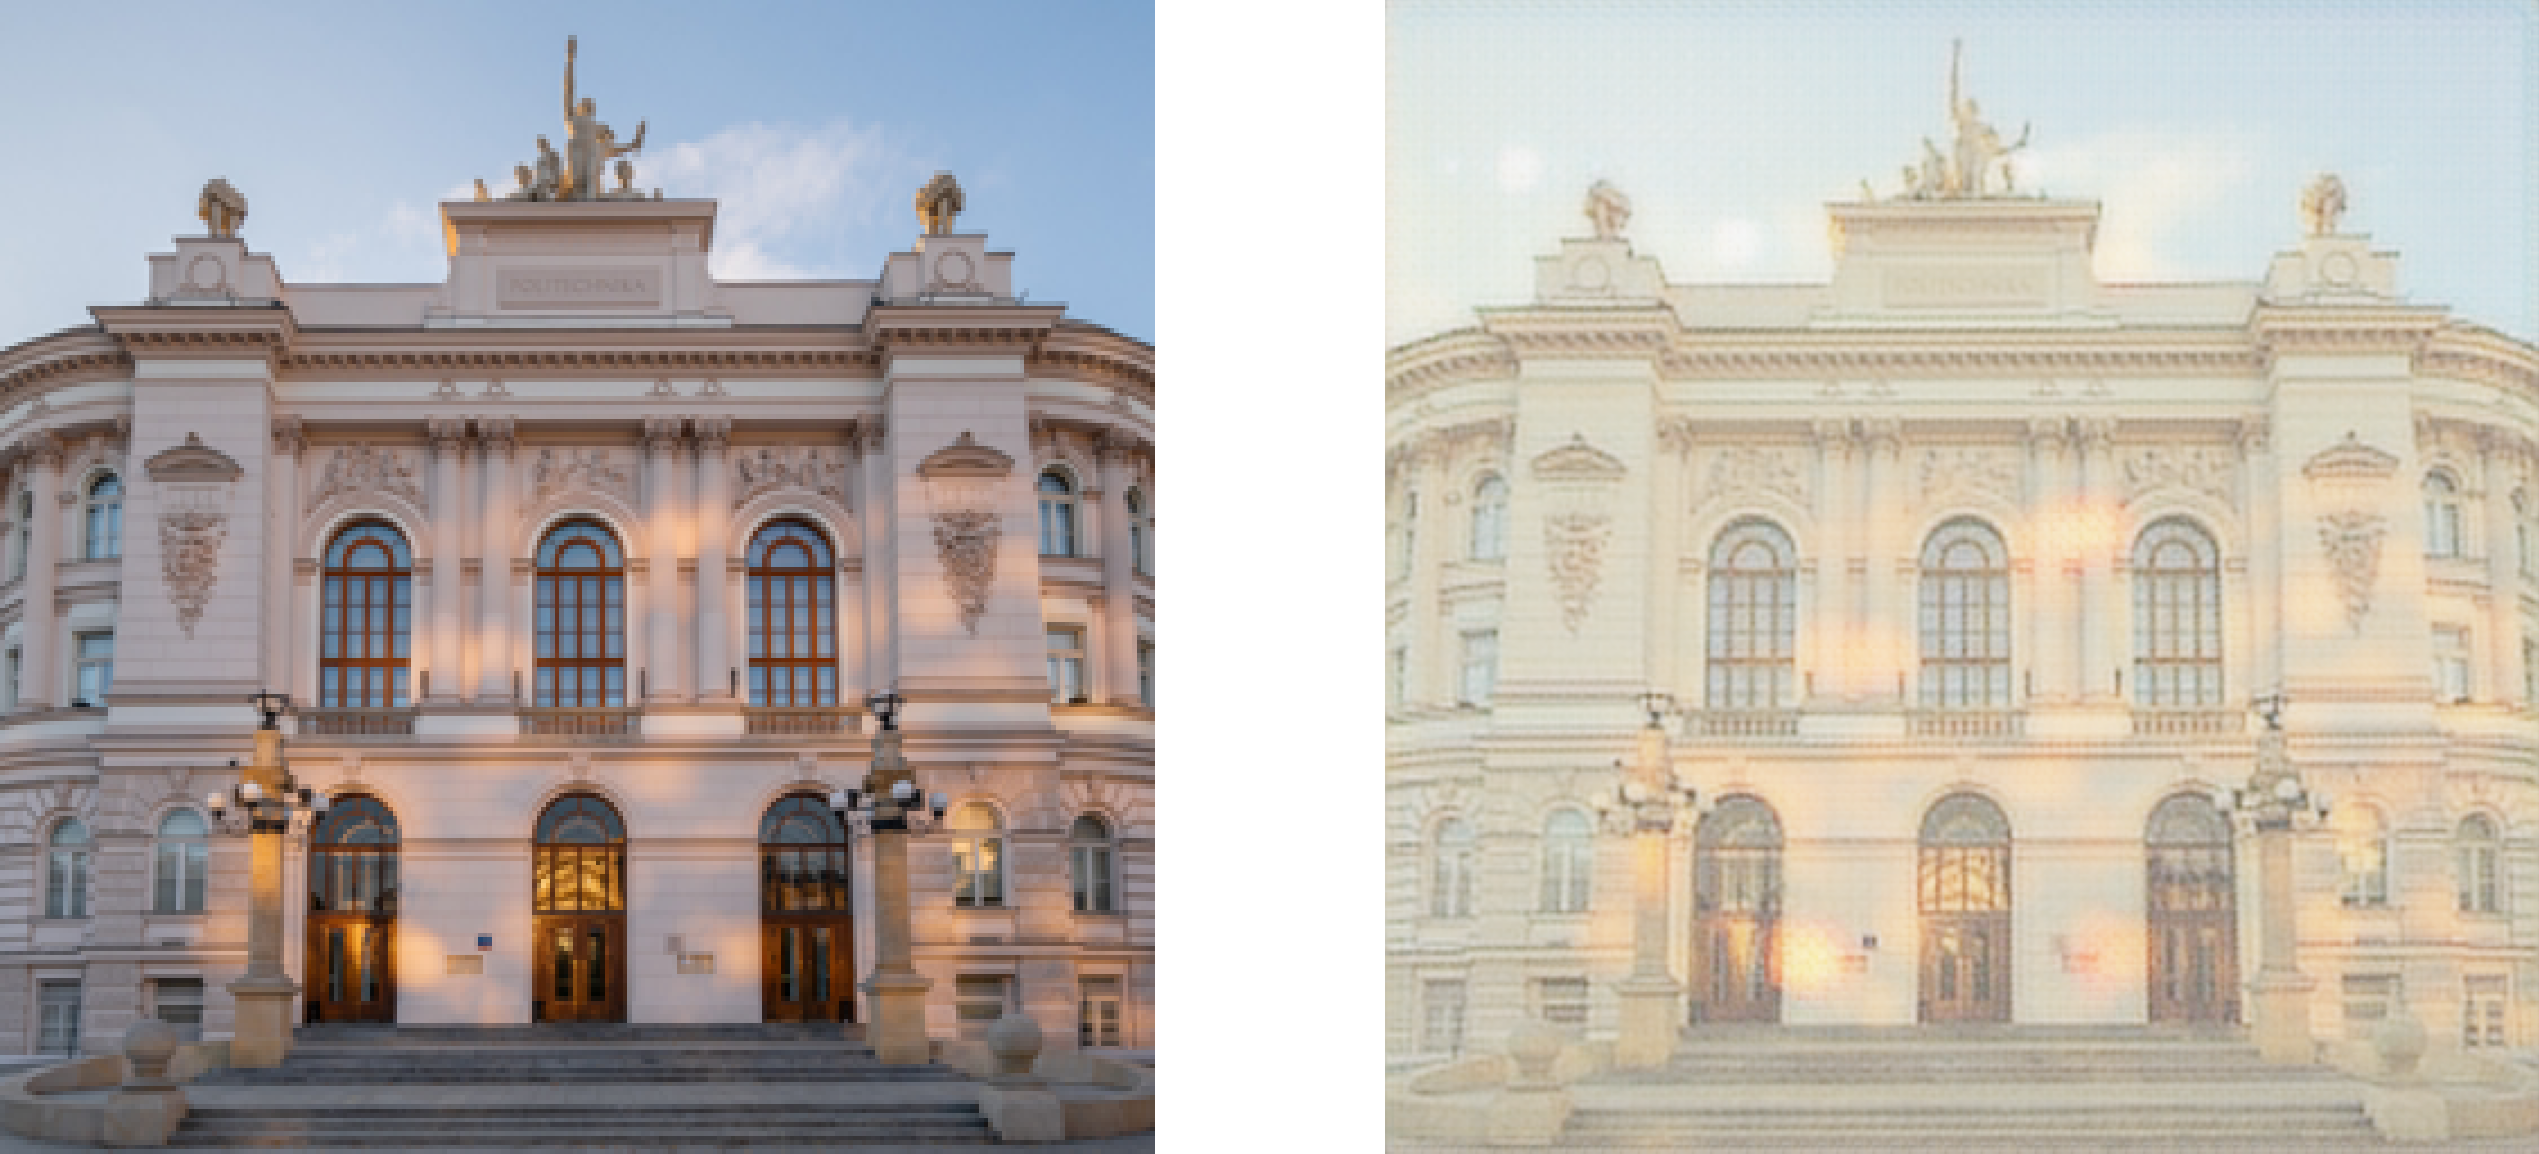
\includegraphics[width=\textwidth]{../imgs/side_by_side/v3.png}

\subsection{Kreskówka}
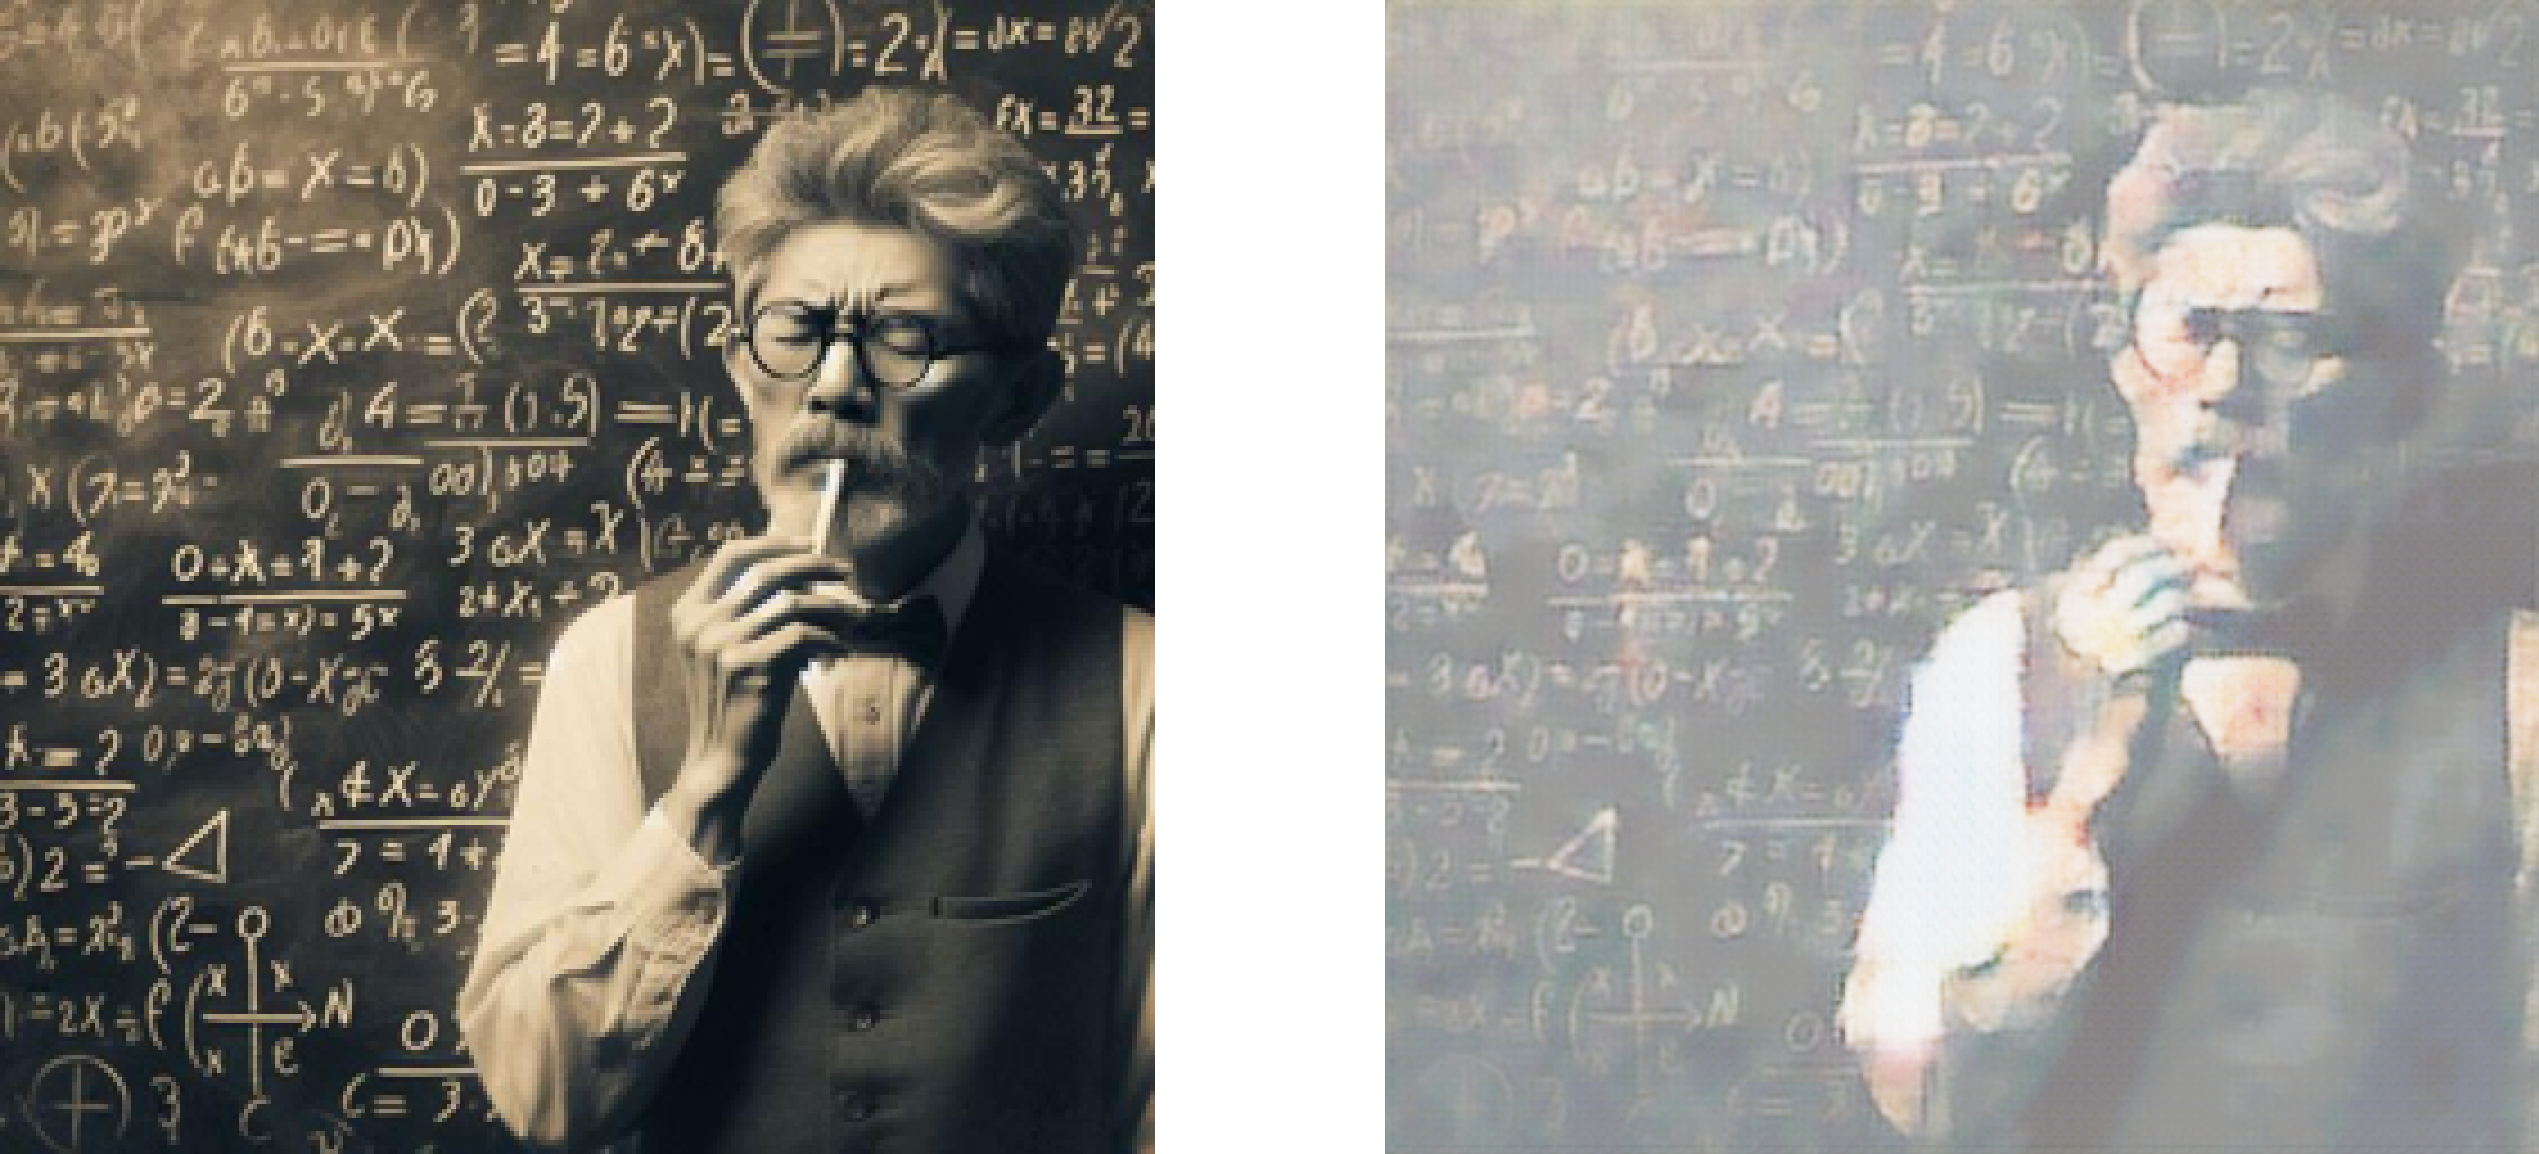
\includegraphics[width=\textwidth]{../imgs/side_by_side/c1.png}
\vspace{3mm} \\
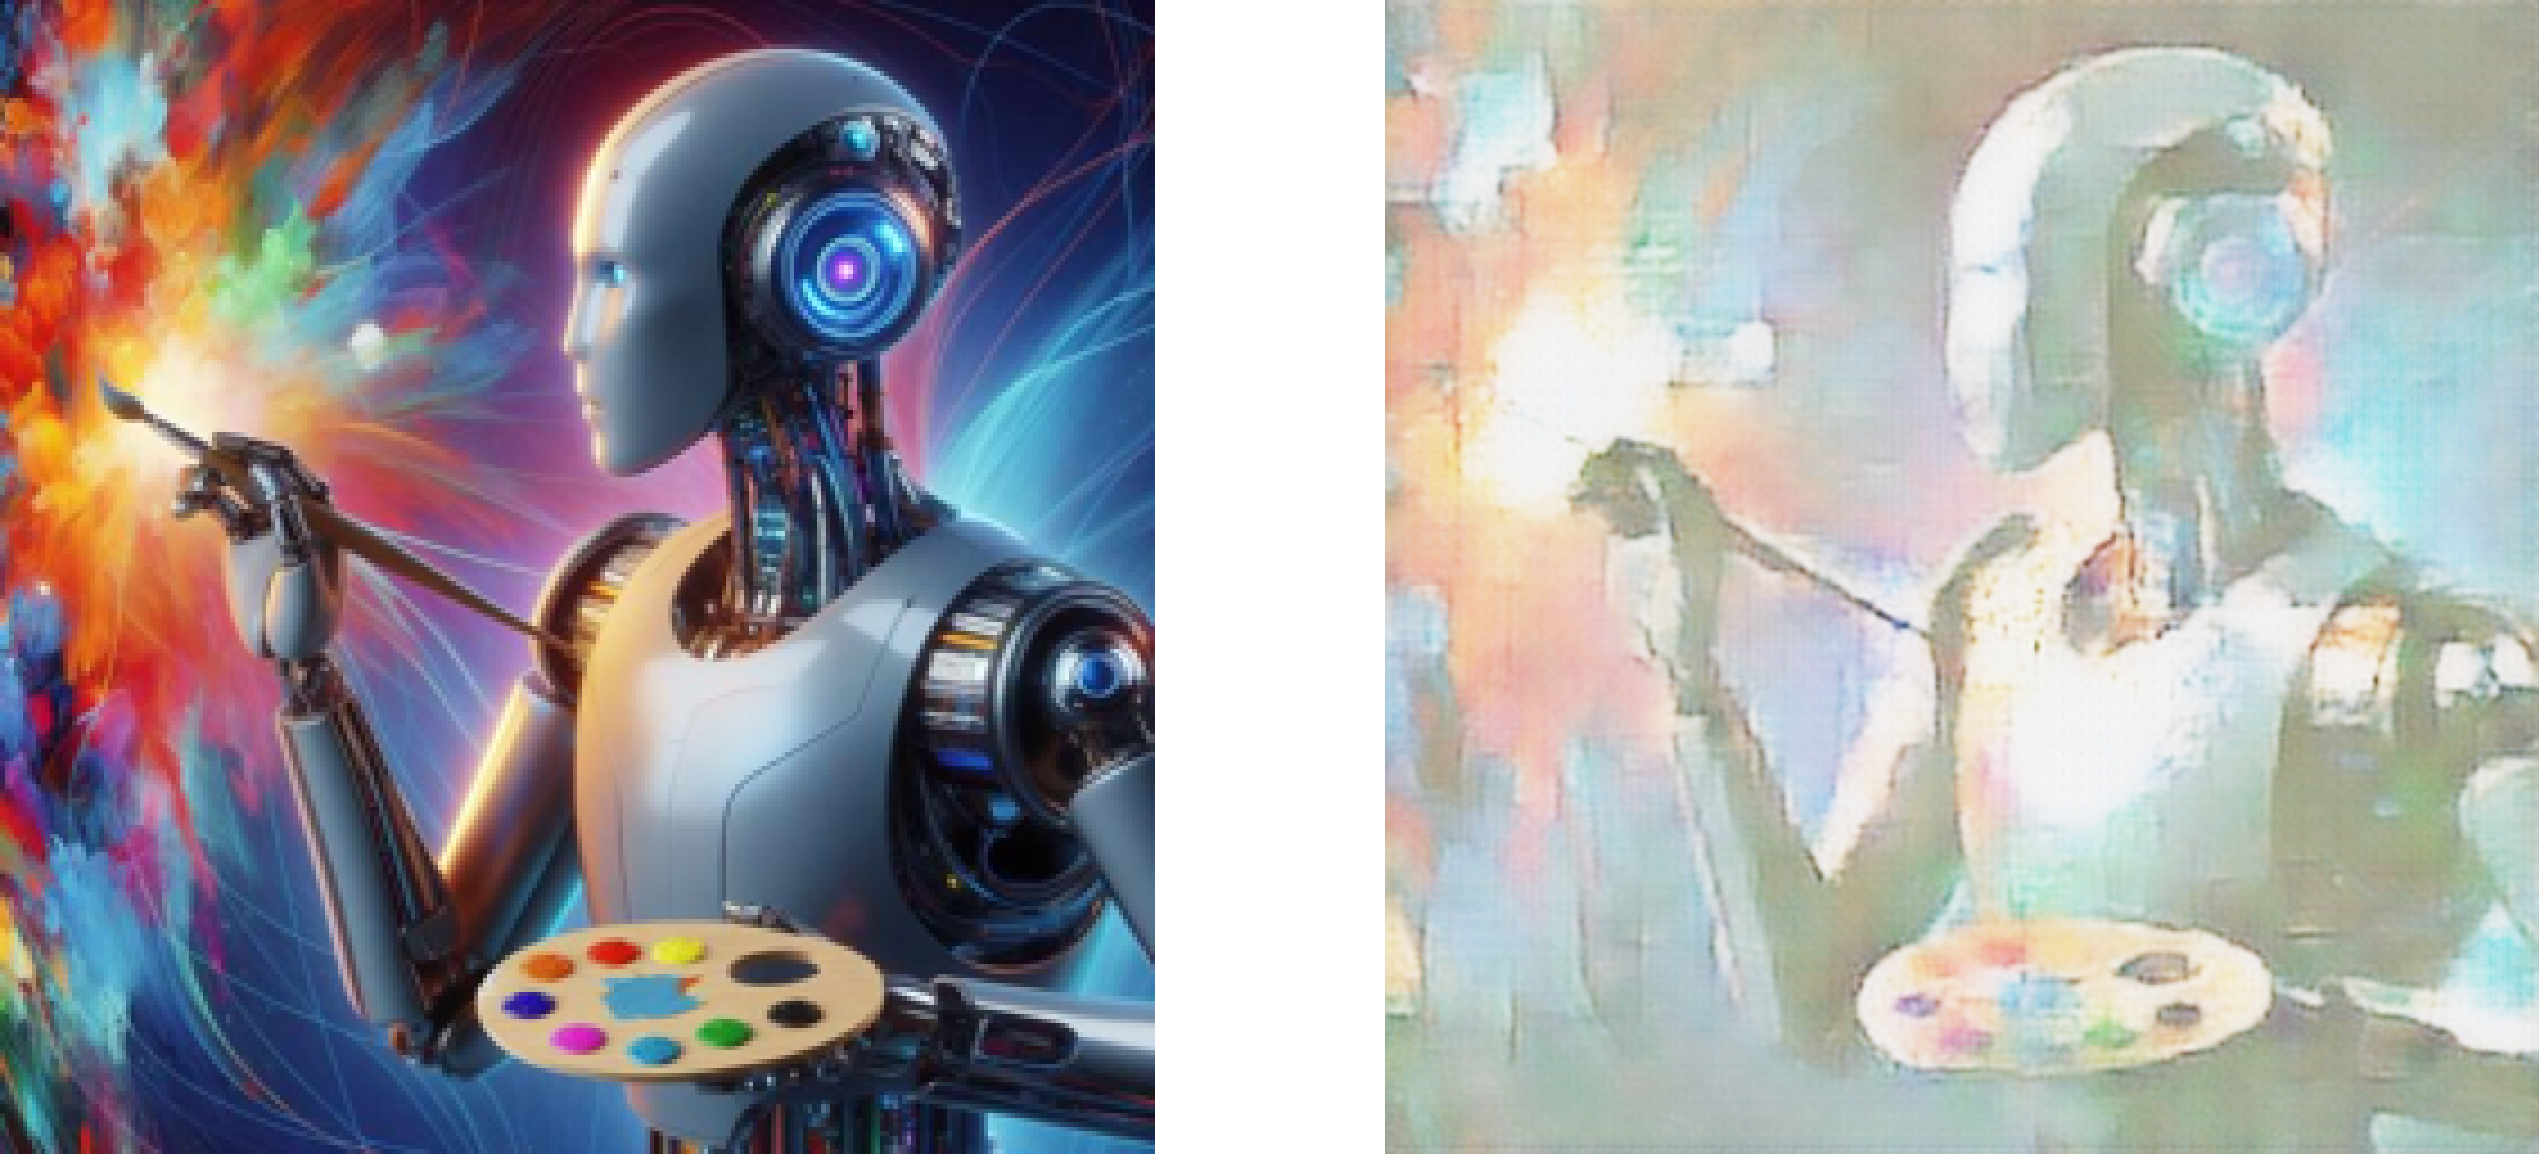
\includegraphics[width=\textwidth]{../imgs/side_by_side/c2.png}
\vspace{3mm} \\
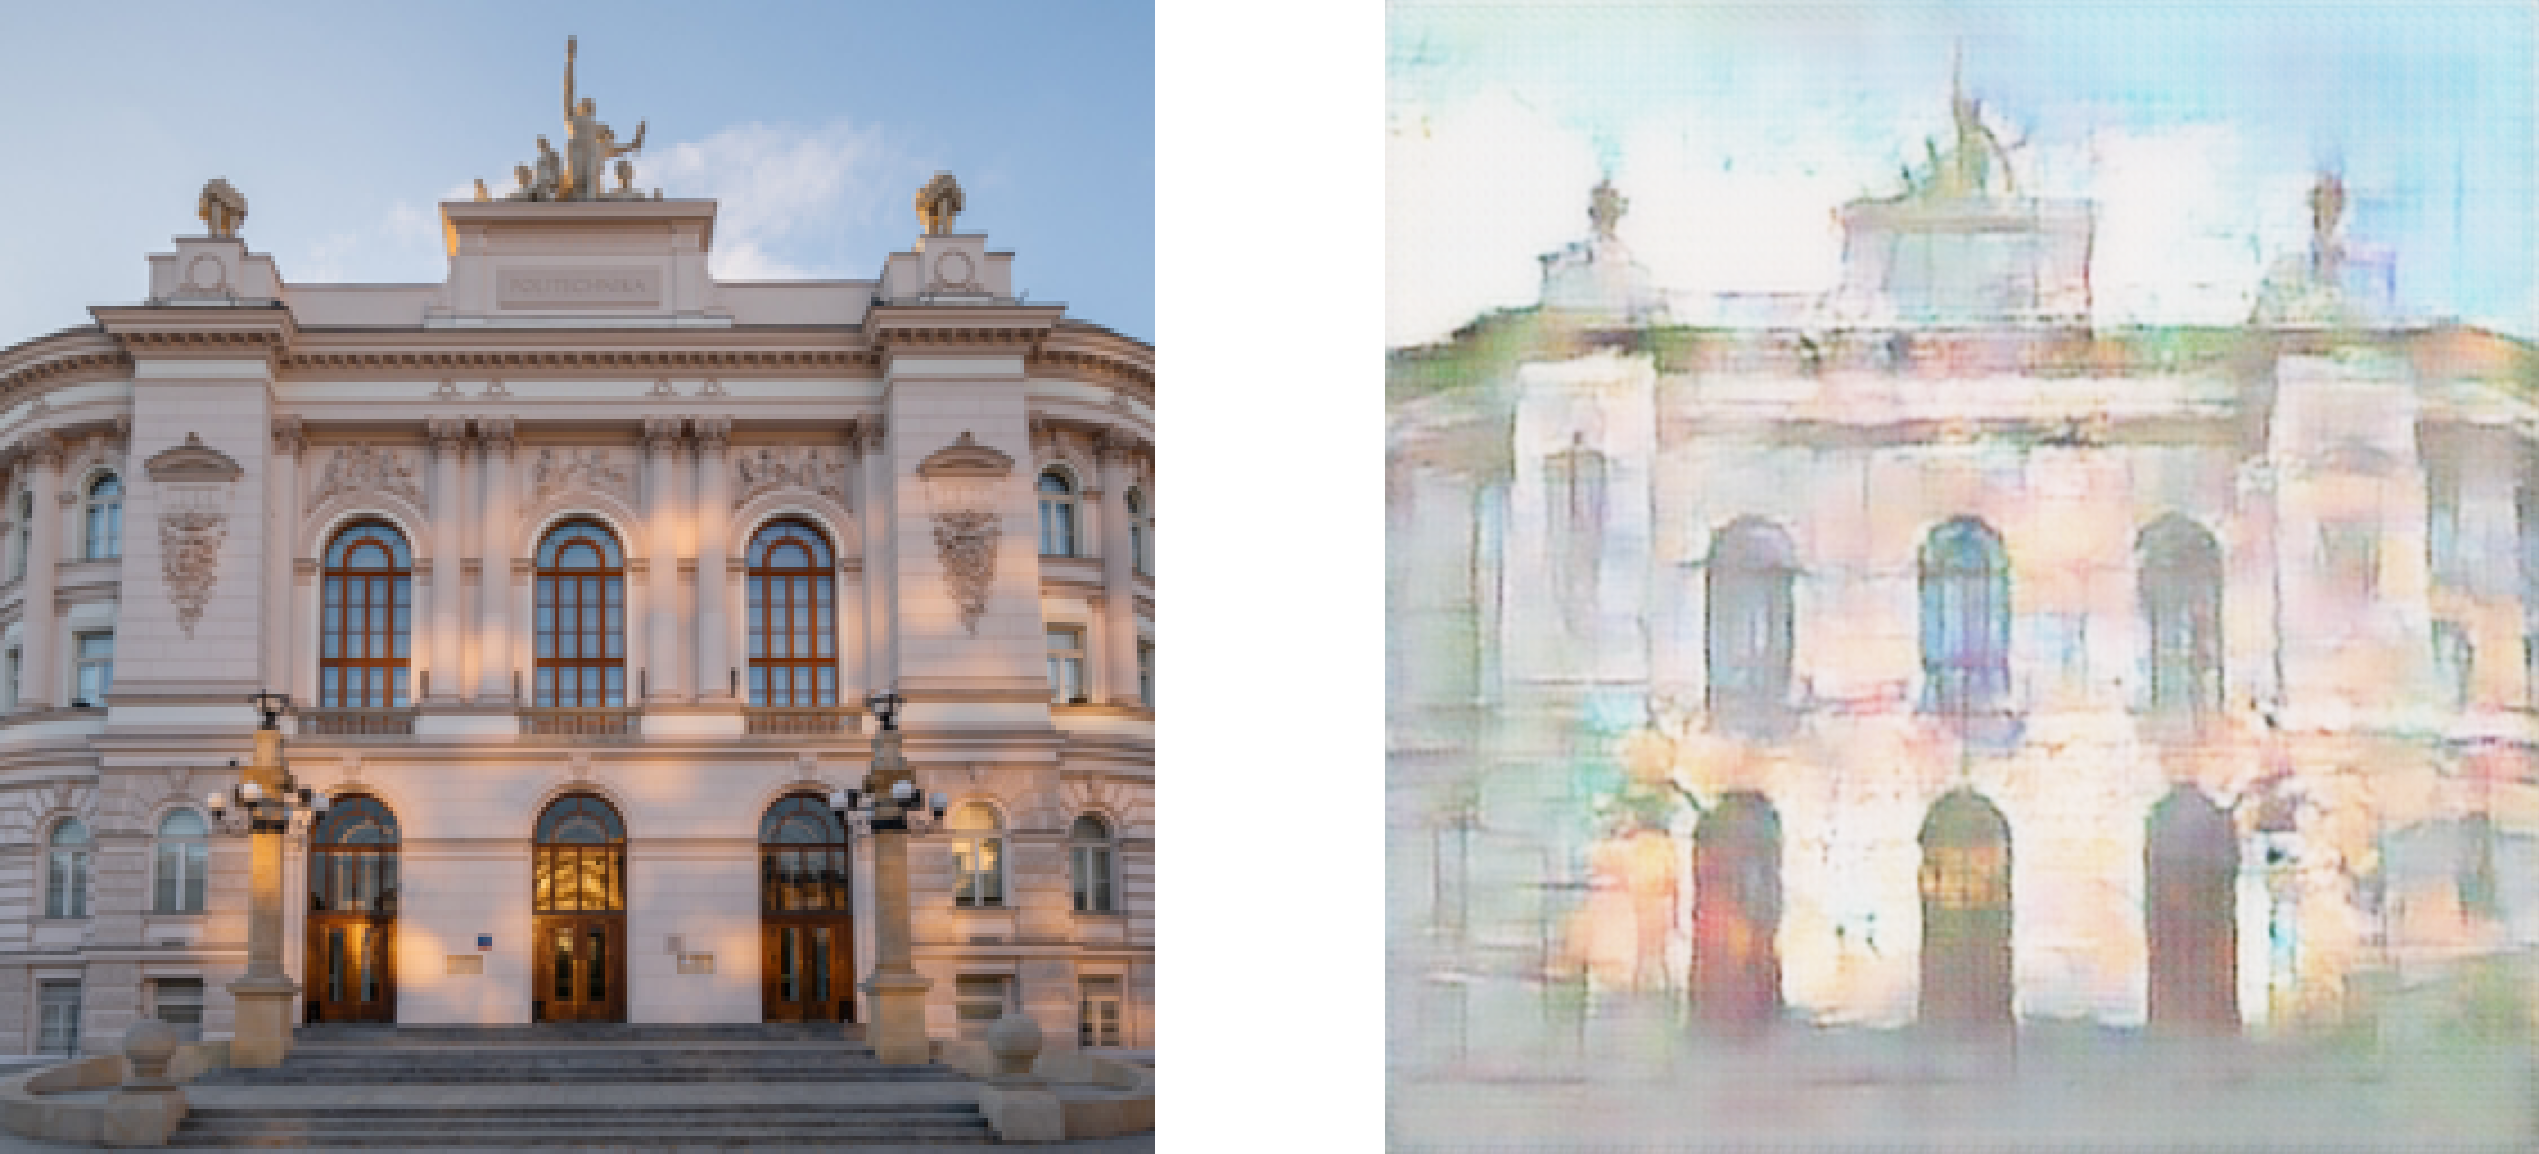
\includegraphics[width=\textwidth]{../imgs/side_by_side/c3.png}

\section{Wnioski}
\begin{itemize}
    \setlength\itemsep{0pt}
    \item Program umożliwia konwersję obrazów na dwa różne style: sztuka Vincenta Van Gogha i kreskówka.
    \item Używa dwóch modeli: CycleGAN do konwersji stylu i SRGAN do skalowania obrazu.
    \item Program został wyposażony w graficzny interfejs, który umożliwia łatwy wybór pliku wejściowego i stylu konwersji.
    \item Aplikacja wymaga dostępności wag modelu, które można uzyskać, uruchamiając notebooki lub pobierając je z podanego linku.
    \item Program działa na systemach operacyjnych Windows i Linux.
    \item Właściwy wybór liczby epok jest kluczowy dla jakości finalnego obrazu. Ważne jest, aby patrzeć na wyniki i monitorować stratę podczas treningu, aby uniknąć przeuczenia.
\end{itemize}

\end{document}